\chapter{Componente tecnologica}
\section{Introduzione}
La realizzazione del progetto prevede, dopo la definizione di una precisa architettura, l'utilizzo di diverse componenti tecnologiche, come ad esempio l'utilizzo di un framework, per soddisfare i vari requisiti utente.
\section{Strumenti utilizzati per l'organizzazione del lavoro}
\subsection{ClickUp}
Ai fini di organizzare per il meglio il lavoro da svolgere, l'utilizzo della piattaforma ClickUp ha permesso al team di sviluppo la suddivisione dei compiti da svolgere mediante la definizione di macro-task, organizzati in dashboard visibili dal settore amministrativo e tecnico. Un macro-task rappresenta l'implementazione di un caso d'uso utente e corrisponde ad un rilascio in produzione. Inoltre prevede un'univocità all'interno della dashboard ed è visibile e modificabile dal reparto di amministrazione per supervisionare l'andamento del progetto. A sua volta un macro-task è suddiviso in task, i quali sono organizzati nei diversi pannelli (admin, negozio, utente, comune) riprendendo il codice univoco a cui è associato il macro-task. Ogni task è inserito nella dashboard gestita dal team di sviluppo e corrisponde all'implementazione di una micro-funzionalità. Deve soddisfare precisi requisiti, di seguito elencati.
\begin{itemize}
    \item \textbf{Durata Limitata}: un task deve prevedere un tempo di implementazione da una alle quattro ore complessive
    \item \textbf{Atomicità}: un task deve prevedere l'implementazione/correzione di funzionalità singole
    \item \textbf{Univocità}: un task non deve essere mai ripetuto, per implementare bugfixes è necessario creare un nuovo macro-task e di seguito organizzarne la suddivisione
    \item \textbf{Reperibilità}: un task deve essere facilmente trovato ricercando parole chiave definite nel titolo, il quale segue lo standard <<\textit{COD \# - Titolo breve}>>
\end{itemize}
Ogni task nel flusso di lavoro può assumere diversi status:
\begin{itemize}
    \item \textbf{Open}: il task è appena stato creato e non è ancora stato implementato
    \item \textbf{In Progress}: il task è in corso di implementazione da parte del team di sviluppo
    \item \textbf{Review}: il task è in corso di revisione da parte dei preposti al testing
    \item \textbf{Closed}: il task è concluso e testato
\end{itemize} 
Un macro-task può passare nello status "closed" solo quando tutti i task a lui relativi sono in closed. A questo punto è possibile procedere con il rilascio della piattaforma in produzione.
\begin{figure}[!htb]
    \centering
    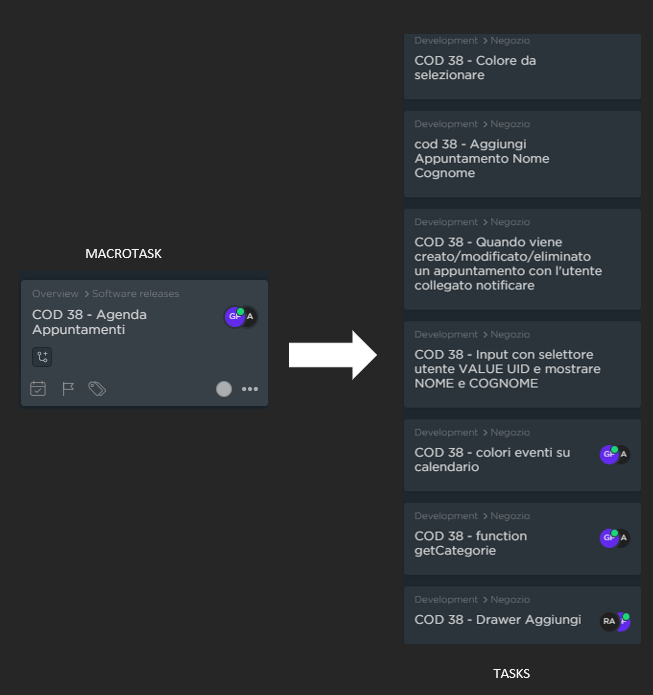
\includegraphics[width=0.7\textwidth]{divis.png}
    \caption{Organizzazione macro-tasks su ClickUp}
\end{figure}
\subsection{Bitbucket}
\subsection{AdobeXD}
\subsection{Separazione ambienti di lavoro}

\section{Javascript e NodeJS}
\subsection{Features introdotte in ES2021 utilizzate}
\subsection{npm}
\newpage
\section{Componente Frontend}
\subsection{Linee guida grafiche per l'interfaccia utente}
\subsection{ReactJS e antd}
\subsection{Less}
\newpage
\section{Componente Backend}
\subsection{Google Cloud}
\subsubsection{Cloud SQL}
\subsubsection{Firebase}
\subsubsection{Firebase Functions}
\subsubsection{Realtime Database}
\subsection{AWS}
\subsubsection{Simple Email Service}
\subsection{Stripe}
\subsubsection{Stripe Connect}